\documentclass{beamer}
\begin{document}

\subsection{Marks for offline examinations}

\begin{frame}{Marks for offline examinations}
	\begin{block}{Problem Statement}
		\begin{itemize}
			\item Several offline exams are conducted in the Bodhi-class model
			\item The marks for these offline exams are usually sent by emails, having CSV files attachments
			\item It is required to have an interface to display these marks to the students on Bodhitree itself
		\end{itemize}
	\end{block}
\end{frame}

\begin{frame}{Specifications}
	\textbf{Instructor Specifications}
	\begin{itemize}
		\item Upload a CSV containing the students marks
		\item The file should have the exam details and marks, along with the usernames of the students, in the following format
	\end{itemize}

	\textbf{Students Specifications}
	\begin{itemize}
		\item Students must be able to view only their marks that are uploaded for the course
	\end{itemize}
	
\end{frame}

\begin{frame}{Design}{User Interface: Instructor}
	\textbf{User Interface as seen by the instructor}
	\begin{figure}
		\centering
		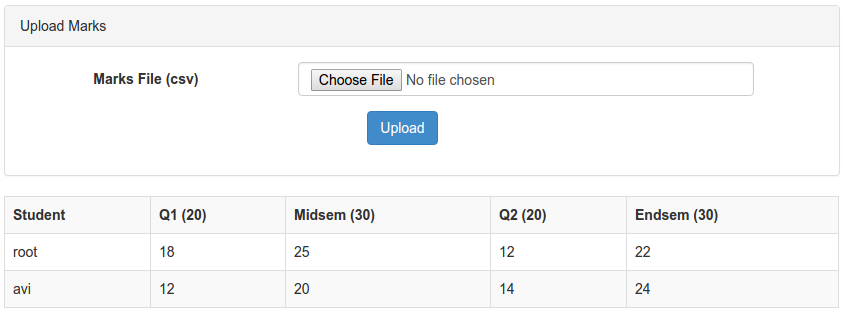
\includegraphics[width=0.8\linewidth]{media/marksi}
		\caption{Instructor's view of CSV upload and display of students marks}
		\label{fig:marksi}
	\end{figure}
\end{frame}

\begin{frame}{Design}{User Interface: Student}
	\textbf{User Interface as seen by the student}
	\begin{figure}
		\centering
		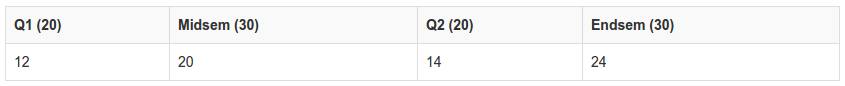
\includegraphics[width=0.8\linewidth]{media/markss1}
		\caption{Student 2's view of his marks}
		\label{fig:markss1}
	\end{figure}
\end{frame}

\begin{frame}{Design}{Upload of marks}
	\textbf{Uploading CSV file}
	
	\begin{center}
		\rowcolors{1}{}{lightgray}
		\bgroup
		\def\arraystretch{1.5}
		\begin{tabular}{ccccc}
			\hline
			\textbf{EXAM\_TYPE} & Q1 & Midsem & Q2 & Endsem \\
			\textbf{MAX\_MARKS} & 20 & 30 & 20 & 30 \\
			Student 1 & 18 & 25 & 12 & 22 \\ 
			Student 2 & 12 & 20 & 14 & 24 \\ 
			\hline 
		\end{tabular}
		\egroup
	\end{center}
		
\end{frame}


\begin{frame}{Design}{Storage of marks}
	\textbf{Storing marks in the database}
	\begin{figure}
		\centering
		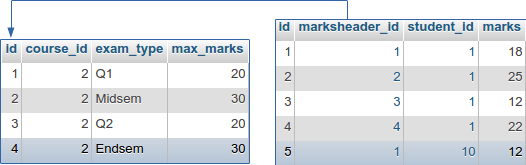
\includegraphics[width=0.8\linewidth]{media/marksdb} \\
		\hspace{1.2cm}Exams details \hspace{1.5cm} Marks obtained by students
		\caption{Data view of the marks module}
		\label{fig:marksdb}
	\end{figure}
	
\end{frame}

\end{document}